\documentclass[a4paper,11pt]{article}
\usepackage{lecturenotes}
\lectureheader{ELE727}{4}
\begin{document}
\tableofcontents
\clearpage
\noteheading{1}{Basic Differential Pair}
\begin{notepanels}[gap=5mm,align=top]
    \begin{notepanel}{}
        \begin{notecircuit}[american,scale=0.75,transform shape,
            font=\Large]{Circuit and bias}
            \ctikzset{current arrow scale=24}
            \tikzset{pair-annotation/.style={NoteAccent,line width=0.3pt,
                -{Latex[length=2pt,width=1.4pt]}}}
            \node[nmos,arrowmos] (M1) at (0,0) {};
            \node[nmos,arrowmos,xscale=-1] (M2) at (3.6,0) {};
            \node[right,inner sep=2pt] at (M1.center) {$M_1$};
            \node[left,inner sep=2pt] at (M2.center) {$M_2$};

            % Matched resistive loads and compact output branches.
            \draw (M1.D) -- ++(0,0.35) coordinate (out1)
                to[R] (M1.D |- 0,3.5) coordinate (dd1);
            \draw (M2.D) -- ++(0,0.35) coordinate (out2)
                to[R] (M2.D |- 0,3.5) coordinate (dd2);
            \draw (dd1) -- (dd2);
            \node[above] at (1.8,3.5) {$V_{DD}$};
            \node at (1.0,2.35) {$R_{D1}$};
            \node at (2.6,2.35) {$R_{D2}$};
            \draw (out1) node[circ] {} -- ++(-0.6,0)
                node[ocirc] {} node[left] {$V_{\mathrm{out1}}$};
            \draw (out2) node[circ] {} -- ++(0.6,0)
                node[ocirc] {} node[right] {$V_{\mathrm{out2}}$};
            \node[right,inner sep=2pt] at (out1) {$X$};
            \node[left,inner sep=2pt] at (out2) {$Y$};

            % The current split is the equal-input bias condition.
            \node[NoteAccent] at (1.8,4.45)
                {$V_{\mathrm{in1}}=V_{\mathrm{in2}}$};
            \draw[pair-annotation] (-0.55,3.05) -- (-0.55,2.45);
            \node[NoteAccent,left,inner sep=5pt] at (-0.55,2.75)
                {$I_{SS}/2$};
            \draw[pair-annotation] (4.15,3.05) -- (4.15,2.45);
            \node[NoteAccent,right,inner sep=5pt] at (4.15,2.75)
                {$I_{SS}/2$};

            % AC signal and DC bias applied to the first input.
            \draw (M1.G) -- (-1.45,0) node[ocirc] {}
                node[above] {$V_{\mathrm{in1}}$} -- (-2.8,0)
                to[sV,l_=$v_{\mathrm{ac}}$] (-2.8,-1.8)
                to[battery1,l_=$V_{\mathrm{DC}}$] (-2.8,-3.0)
                -- (-2.8,-3.15) node[ground] {};
            \draw (M2.G) -- ++(0.6,0) node[ocirc] {}
                node[right] {$V_{\mathrm{in2}}$};

            % Common source node and ideal tail-current sink.
            \draw (M1.S) -- (M1.S |- 0,-1.05)
                -- (1.8,-1.05) coordinate (tail)
                -- (M2.S |- 0,-1.05) -- (M2.S);
            \draw (tail) node[circ] {} to[I,l=$I_{SS}$] (1.8,-2.95)
                -- (1.8,-3.1) node[ground] {};
            \node[below right,inner sep=2pt,NoteAccent] at (tail) {$V_{SS}$};

            % Gate-to-source polarities are kept clear of the device labels.
            \node[NoteAccent] at (-0.85,-0.33) {$+$};
            \node[NoteAccent] at (-0.85,-1.05) {$-$};
            \node[NoteAccent,left,inner sep=3pt] at (-0.85,-0.69) {$V_{GS1}$};
            \node[NoteAccent] at (4.45,-0.33) {$+$};
            \node[NoteAccent] at (4.45,-1.05) {$-$};
            \node[NoteAccent,right,inner sep=3pt] at (4.45,-0.69) {$V_{GS2}$};

            \draw[pair-annotation] (0.55,-3.65) -- (1.35,-2.35);
            \node[NoteAccent,align=center,anchor=north] at (1.0,-3.8)
                {$I_{SS}$ independent of $V_{\mathrm{in,CM}}$\\[-1pt]
                 {\sffamily (another transistor)}};
            \node[NoteAccent] at (1.0,-5.3) {$V_{GS1}=V_{\mathrm{DC}}-V_{SS}$};
            \node at (1.0,-6.1) {$R_{D1}=R_{D2}=R_D$};
        \end{notecircuit}
    \end{notepanel}
    \begin{notepanel}{}
        \begin{center}
        {\sffamily\small\bfseries\color{NoteMuted}Single-ended outputs\par}
        \vspace{3mm}
        \begin{tikzpicture}[x=12mm,y=7mm,font=\scriptsize,
            color=NoteInk,
            pair-axis/.style={NoteMuted,line width=0.4pt,
                -{Latex[length=3pt,width=2.3pt]}},
            pair-guide/.style={NoteAccent,densely dashed,line width=0.35pt}]
            \draw[pair-axis] (-1.8,0) -- (1.85,0);
            \draw[pair-axis] (0,-0.1) -- (0,3.15);
            \draw[NoteRule,densely dotted] (-1.8,1.7) -- (1.85,1.7);
            \draw[pair-guide] (-1,0.65) -- (-1,2.95);
            \draw[pair-guide] (1,0.65) -- (1,2.95);

            % Square-law MOS current steering, with full-current end limits.
            \draw[thick] (-1.65,2.5) -- (-1,2.5)
                plot[domain=-1:1,samples=81] (\x,{1.7-0.8*\x*sqrt(2-\x*\x)})
                -- (1.65,0.9);
            \draw[thick,NoteAccent] (-1.65,0.9) -- (-1,0.9)
                plot[domain=-1:1,samples=81] (\x,{1.7+0.8*\x*sqrt(2-\x*\x)})
                -- (1.65,2.5);
            \node[above] at (-1.45,2.5) {$V_{\mathrm{out1}}$};
            \node[below,NoteAccent] at (-1.45,0.9) {$V_{\mathrm{out2}}$};
            \node[above left,inner sep=2pt] at (-1.65,2.5) {$V_{DD}$};
            \node[below left,inner sep=2pt] at (-1.65,0.9) {$V_{DD}-R_DI_{SS}$};
            \node[left,inner sep=3pt] at (-1.8,1.7) {$V_{\mathrm{out,CM}}$};
            \node[right,fill=white,inner sep=2pt] at (0.55,1.7)
                {$V_{DD}-\dfrac{R_DI_{SS}}{2}$};
            \fill[NoteAccent] (0,1.7) circle[radius=1.5pt];
            \draw[NoteAccent,line width=0.3pt,
                -{Latex[length=2pt,width=1.4pt]}] (0.7,0.5) -- (0.03,1.65);
            \node[NoteAccent,right,inner sep=2pt] at (0.75,0.5)
                {$V_{\mathrm{in1}}=V_{\mathrm{in2}}$};
            \node[above,NoteAccent] at (-1,2.95) {$M_1$ off};
            \node[above,NoteAccent] at (1,2.95) {$M_2$ off};
            \node[below,inner sep=3pt] at (1.75,0)
                {$V_{\mathrm{in1}}-V_{\mathrm{in2}}$};
        \end{tikzpicture}\par
        {\scriptsize\color{NoteAccent}
            $M_2$ may enter triode at the left limit.\par
            $\Delta V_{\mathrm{in1}}=-\Delta V_{\mathrm{in2}}$\par}

        \vspace{2.6mm}
        {\sffamily\small\bfseries\color{NoteMuted}Differential output\par}
        \vspace{4mm}
        \begin{tikzpicture}[x=12mm,y=8mm,font=\scriptsize,
            color=NoteInk,
            pair-axis/.style={NoteMuted,line width=0.4pt,
                -{Latex[length=3pt,width=2.3pt]}}]
            \fill[NoteTint] (-1,-1.15) rectangle (1,1.15);
            \draw[NoteAccent,densely dashed,line width=0.35pt]
                (-1,-1.2) -- (-1,1.2) (1,-1.2) -- (1,1.2);
            \draw[pair-axis] (-1.8,0) -- (1.85,0);
            \draw[pair-axis] (0,-1.3) -- (0,1.4);
            \draw[thick] (-1.65,1) -- (-1,1)
                plot[domain=-1:1,samples=81] (\x,{-\x*sqrt(2-\x*\x)})
                -- (1.65,-1);
            \node[left,inner sep=3pt] at (-1.65,1) {$+R_DI_{SS}$};
            \node[right,inner sep=3pt] at (1.65,-1) {$-R_DI_{SS}$};
            \node[above,inner sep=4pt] at (0,1.4)
                {$V_{\mathrm{out1}}-V_{\mathrm{out2}}$};
            \node[below,inner sep=3pt] at (1.75,0)
                {$V_{\mathrm{in1}}-V_{\mathrm{in2}}$};
            \draw[NoteAccent,line width=0.4pt]
                (-1,-1.3) -- (-1,-1.42) -- (1,-1.42) -- (1,-1.3);
            \node[below,NoteAccent,inner sep=4pt] at (0,-1.42)
                {$M_1,M_2$ in saturation};
        \end{tikzpicture}
        \end{center}
    \end{notepanel}
\end{notepanels}
\noteheading{2}{Common-mode}
\begin{notecircuit}[american,scale=0.55,transform shape,
    font=\Large]{Common-mode differential pair}
    \node[nmos,arrowmos] (CM1) at (0,0) {};
    \node[nmos,arrowmos,xscale=-1] (CM2) at (2.8,0) {};
    \node[nmos,arrowmos,anchor=D] (CM3) at (1.4,-1.65) {};
    \node[right,inner sep=2pt] at (CM1.center) {$M_1$};
    \node[left,inner sep=2pt] at (CM2.center) {$M_2$};
    \node[right,inner sep=2pt] at (CM3.center) {$M_3$};
    \coordinate (cm-left) at ($(CM1.G)+(-0.35,0)$);
    \coordinate (cm-right) at ($(CM2.G)+(0.35,0)$);

    % Highlight the shared input; the bridge keeps it separate from the tail.
    \draw[yellow!65,line width=4pt,line cap=round,line join=round]
        (cm-left) -- (cm-left |- 0,-1.35) -- (1.24,-1.35)
        arc[start angle=180,end angle=0,radius=0.16]
        -- (cm-right |- 0,-1.35) -- (cm-right) -- (CM2.G);

    \draw (CM1.D) -- ++(0,0.25) coordinate (cm-out1)
        to[R] (CM1.D |- 0,2.65) coordinate (cm-dd1);
    \draw (CM2.D) -- ++(0,0.25) coordinate (cm-out2)
        to[R] (CM2.D |- 0,2.65) coordinate (cm-dd2);
    \draw (cm-dd1) -- (cm-dd2) -- ++(0.25,0)
        node[right] {$V_{DD}$};
    \node at (0.95,1.85) {$R_D$};
    \node at (1.85,1.85) {$R_D$};
    \draw (cm-out1) node[circ] {} -- ++(-0.45,0)
        node[ocirc] {} node[left] {$V_{\mathrm{out1}}$};
    \draw (cm-out2) node[circ] {} -- ++(0.45,0)
        node[ocirc] {} node[right] {$V_{\mathrm{out2}}$};
    \node[right,inner sep=2pt] at (cm-out1) {$X$};
    \node[left,inner sep=2pt] at (cm-out2) {$Y$};

    \draw (CM1.S) -- (CM1.S |- 0,-0.9)
        -- (1.4,-0.9) coordinate (cm-tail)
        -- (CM2.S |- 0,-0.9) -- (CM2.S);
    \draw (cm-tail) node[circ] {} -- (CM3.D);
    \node[above,inner sep=2pt] at (cm-tail) {$P$};
    \draw (CM3.S) -- ++(0,-0.18) node[ground] {};
    \draw (CM3.G) -- ++(-0.4,0) node[circ] {}
        node[left] {$V_b$};

    \draw (CM1.G) -- (cm-left) node[circ] {} -- ++(-0.35,0)
        node[ocirc] {} node[left] {$V_{\mathrm{in,CM}}$};
    \draw (cm-left) -- (cm-left |- 0,-1.35) -- (1.24,-1.35);
    \draw[preaction={draw=white,line width=2pt}]
        (1.24,-1.35) arc[start angle=180,end angle=0,radius=0.16];
    \draw (1.56,-1.35) -- (cm-right |- 0,-1.35)
        -- (cm-right) -- (CM2.G);
\end{notecircuit}

Determining the various states of the transistors in the circuit.
\begin{itemize}
    \item M3 is on when $V_{B} > V_{Th_{3}}$
    \item \textcolor{red}{$V_{in,CM} < V_{th}$}:, both M1 \& M2 are off \begin{itemize}
        \item Therefore P is at 0 voltage, and M3 can be modelled as a equivalent resistor with resistance: $r_{o,3}$
        \item $V_{out_{1}} = V_{out_{2}} = V_{dd}$
    \end{itemize}
    \item \textcolor{red}{$V_{in,cm} = V_{th}$}: M1 \& M2 are on and in saturation. \begin{itemize}
        \item $V_{p}$ begins to increase
        \item M3 is in triode
        \item $V_{in,CM} = V_{DD}$
    \end{itemize}
\end{itemize}
\begin{notederivation}[mode=steps, explanation=beside]{M3 Saturation Condition}
    \derivestep{V_{p} = V_{in,cm} - V_{gs_{1}} \gg  V_{ov_{3}}}{Saturation condition for M3}
    \derivestep{I_{1} = I_{2} = \frac{I_{3}}{2}}{Current relation via schematic}
    \derivestep{V_{out_{1,2}} = V_{dd} - \frac{I_{3}}{2} \cdot R_{D}}{Simple voltage drop between $V_{dd} \& V_{out_{1,2}}$}
    \derivestep{V_{dd} - \frac{I_{3}}{2} \cdot R_{B} \gg  V_{DD} - V_{th_{1}} \to \frac{I_{ss}}{2} . R_{D} \leq  V_{th_{1}}}{Final condition for saturation}
\end{notederivation}

\noteheading{2}{Differential Gain}

We can derive differential gain via two approaches: 1) Superposition, and 2) Half-circuit analysis. Superposition however takes too long for more complex 
circuits.

\noteheading{3}{Superposition}
\notedefinition{Superposition}{Turn off a source, replace the source with an equivalent circuit looking into the source}
\par\addvspace{7pt}
\noindent\begin{minipage}{\linewidth}
    \centering
    \captionsetup{hypcap=false,type=figure}
    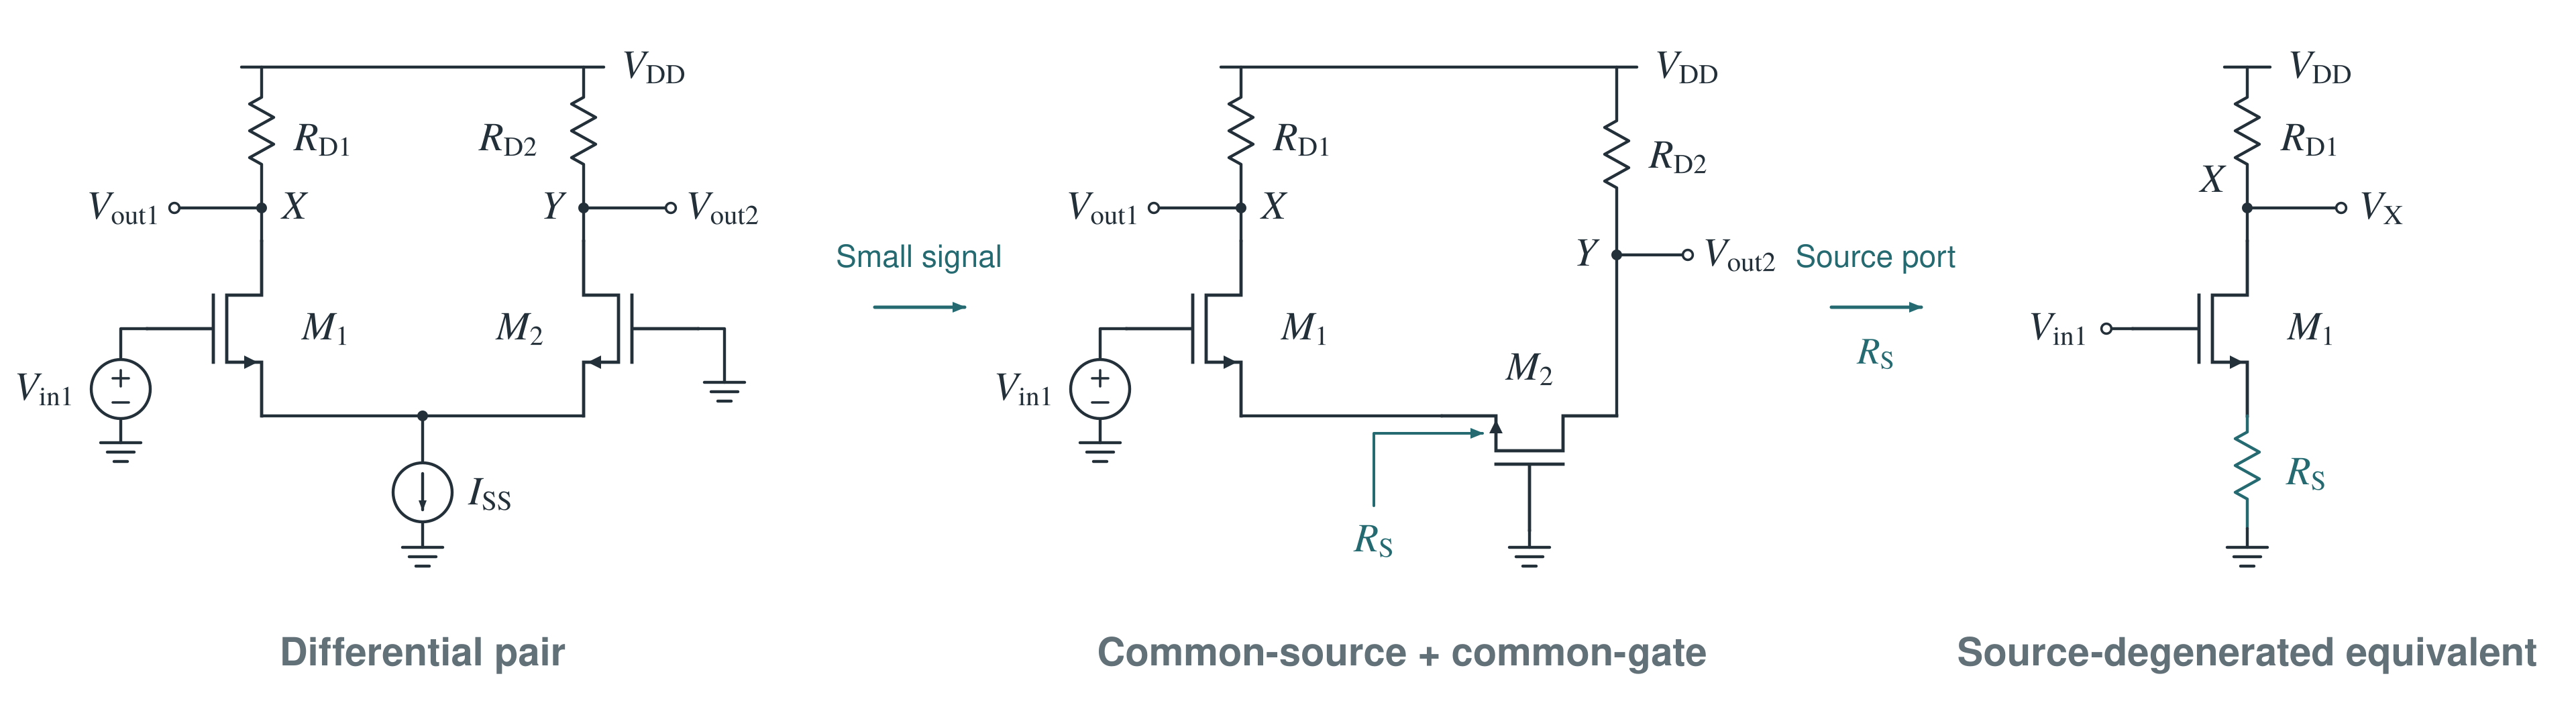
\includegraphics[width=0.8\linewidth,keepaspectratio]{figures/differential-pair-circuit-composition.png}
    \caption{Example of Superposition for the Simple Differential Pair}
    \label{fig:}
\end{minipage}
\par\addvspace{7pt}
\noteheading{3}{Half-circuit}
\assumption{Perfect symmetry: $g_{m1}=g_{m2}$ and $R_{D1}=R_{D2}$.}
\begin{notederivation}[mode=steps,explanation=beside]{Small-signal changes}
    \derivestep{\Delta V_{\mathrm{in1}}=-\Delta V_{\mathrm{in2}}=\Delta V}
        {Equal and opposite input changes.}
    \derivestep{\Delta I_{D1}=-\Delta I_{D2}=\Delta I}
        {Small, equal and opposite drain-current changes.}
    \derivestep{\Delta V_P=0}
        {No change at node $P$: AC ground.}
\end{notederivation}
\begin{center}
\begin{minipage}{0.70\linewidth}
\begin{notepanels}[widths={1.3,1},gap=5mm,align=center]
\begin{notepanel}{}
\begin{notecircuit}[american,scale=0.5,transform shape,
    font=\Large]{Differential excitation}
    \ctikzset{current arrow scale=24}
    \tikzset{diff-current/.style={NoteAccent,line width=0.3pt,
        -{Latex[length=2pt,width=1.4pt]}}}
    \node[nmos,arrowmos] (DP1) at (0,0) {};
    \node[nmos,arrowmos,xscale=-1] (DP2) at (3.6,0) {};
    \node[right,inner sep=2pt] at (DP1.center) {$M_1$};
    \node[left,inner sep=2pt] at (DP2.center) {$M_2$};

    \draw (DP1.D) -- ++(0,0.45) coordinate (diff-out1)
        to[R] (DP1.D |- 0,3.1) coordinate (diff-dd1);
    \draw (DP2.D) -- ++(0,0.45) coordinate (diff-out2)
        to[R] (DP2.D |- 0,3.1) coordinate (diff-dd2);
    \draw (diff-dd1) -- (diff-dd2);
    \node[above,inner sep=4pt] at (1.8,3.1) {$V_{DD}$};
    \node at (1.0,2.1) {$R_{D1}$};
    \node at (2.6,2.1) {$R_{D2}$};
    \draw (diff-out1) node[circ] {} -- ++(-0.65,0)
        node[ocirc] {} node[left] {$V_{\mathrm{out1}}$};
    \draw (diff-out2) node[circ] {} -- ++(0.65,0)
        node[ocirc] {} node[right] {$V_{\mathrm{out2}}$};
    \node[right,inner sep=5pt] at (diff-out1) {$X$};
    \node[left,inner sep=5pt] at (diff-out2) {$Y$};

    % Equal and opposite changes at the two gates.
    \draw (DP1.G) -- ++(-0.55,0) coordinate (diff-in1) node[ocirc] {};
    \draw (DP2.G) -- ++(0.55,0) coordinate (diff-in2) node[ocirc] {};
    \node[left,align=right,inner sep=6pt] at (diff-in1)
        {$V_{\mathrm{in1}}$\\[2pt]\color{NoteAccent}$+\Delta V$};
    \node[right,align=left,inner sep=6pt] at (diff-in2)
        {$V_{\mathrm{in2}}$\\[2pt]\color{NoteAccent}$-\Delta V$};
    \draw[diff-current] (-0.55,2.7) -- (-0.55,2.1);
    \node[left,inner sep=7pt,NoteAccent] at (-0.55,2.4) {$+\Delta I$};
    \draw[diff-current] (4.15,2.7) -- (4.15,2.1);
    \node[right,inner sep=7pt,NoteAccent] at (4.15,2.4) {$-\Delta I$};

    \draw (DP1.S) -- (DP1.S |- 0,-1.0)
        -- (1.8,-1.0) coordinate (diff-tail)
        -- (DP2.S |- 0,-1.0) -- (DP2.S);
    \draw (diff-tail) node[circ] {} to[I,l=$I_{SS}$] (1.8,-2.55)
        -- (1.8,-2.7) node[ground] {};
    \node[anchor=north] at (1.8,-3.45) {$R_{D1}=R_{D2}=R_D$};
\end{notecircuit}
\end{notepanel}
\begin{notepanel}{}
    {\color{NoteAccent}
    \[
        \begin{aligned}
            I_1 &= \frac{I_{SS}}{2}+\Delta I\\[7pt]
            I_2 &= \frac{I_{SS}}{2}-\Delta I
        \end{aligned}
    \]}
\end{notepanel}
\end{notepanels}
\end{minipage}
\end{center}

\noteheading{3}{Deriving Differential Gain using Half-circuit Analysis}
% \assu
\par\noindent\begin{minipage}{\linewidth}
\begin{notecircuit}[american,scale=0.55,transform shape,
    font=\Large]{Virtual-ground decomposition}
    \node[nmos,arrowmos] (HG1) at (0,0) {};
    \node[nmos,arrowmos,xscale=-1] (HG2) at (3.6,0) {};
    \node[right,inner sep=2pt] at (HG1.center) {$M_1$};
    \node[left,inner sep=2pt] at (HG2.center) {$M_2$};
    \draw (HG1.D) -- ++(0,0.4) coordinate (hg-out1)
        to[R] (HG1.D |- 0,3.0) coordinate (hg-dd1);
    \draw (HG2.D) -- ++(0,0.4) coordinate (hg-out2)
        to[R] (HG2.D |- 0,3.0) coordinate (hg-dd2);
    \draw (hg-dd1) -- (hg-dd2);
    \node[above,inner sep=4pt] at (1.8,3.0) {$V_{DD}$};
    \node at (1.0,2.05) {$R_{D1}$};
    \node at (2.6,2.05) {$R_{D2}$};
    \draw (hg-out1) node[circ] {} -- ++(-0.55,0)
        node[ocirc] {} node[left] {$V_{\mathrm{out1}}$};
    \draw (hg-out2) node[circ] {} -- ++(0.55,0)
        node[ocirc] {} node[right] {$V_{\mathrm{out2}}$};
    \node[right,inner sep=5pt] at (hg-out1) {$X$};
    \node[left,inner sep=5pt] at (hg-out2) {$Y$};
    \draw (HG1.G) -- (-1.85,0)
        to[V,l_=$+V_{\mathrm{in1}}$] (-1.85,-1.7)
        -- (-1.85,-1.9) node[ground] {};
    \draw (HG2.G) -- (5.45,0)
        to[V,l=$-V_{\mathrm{in1}}$] (5.45,-1.7)
        -- (5.45,-1.9) node[ground] {};
    % The common source is a virtual AC ground, split into two half-circuits.
    \draw (HG1.S) -- (HG1.S |- 0,-1.0)
        -- (1.2,-1.0) -- (1.2,-1.2) node[ground] {};
    \draw (HG2.S) -- (HG2.S |- 0,-1.0)
        -- (2.4,-1.0) -- (2.4,-1.2) node[ground] {};
\end{notecircuit}
\begin{center}
\begin{minipage}{0.82\linewidth}
\begin{notepanels}[widths={1,1.2},gap=8mm,align=top]
    \begin{notepanel}{}
        \begin{notecircuit}[american,scale=0.55,transform shape,
            font=\Large]{Common-source half-circuit}
            \node[nmos,arrowmos] (HC) at (0,0) {};
            \node[right,inner sep=2pt] at (HC.center) {$M_1$};
            \draw (HC.D) to[R] (HC.D |- 0,2.7) coordinate (hc-dd);
            \draw (hc-dd) ++(-0.25,0) -- ++(0.5,0);
            \node[above,inner sep=4pt] at (hc-dd) {$V_{DD}$};
            \node[right] at (0.45,1.75) {$R_{D1}$};
            \draw (HC.G) -- ++(-0.45,0)
                node[ocirc] {} node[left] {$V_{\mathrm{in1}}$};
            \draw (HC.S) -- ++(0,-0.2) node[ground] {};
        \end{notecircuit}
    \end{notepanel}
    \begin{notepanel}{}
        \begin{notecircuit}[american,scale=0.55,transform shape,
            font=\Large]{Differential-input model}
            \node[nmos,arrowmos] (DI1) at (0,0) {};
            \node[nmos,arrowmos,xscale=-1] (DI2) at (2.8,0) {};
            \node[right,inner sep=2pt] at (DI1.center) {$M_1$};
            \node[left,inner sep=2pt] at (DI2.center) {$M_2$};
            \draw (DI1.D) -- ++(0,0.55) node[ocirc] {};
            \draw (DI2.D) -- ++(0,0.55) node[ocirc] {};
            \draw (DI1.S) -- (DI1.S |- 0,-1.0)
                -- (DI2.S |- 0,-1.0) -- (DI2.S);
            \draw (DI1.G) -- (-1.55,0)
                to[sV,l_=$V_{id}$] (-1.55,-1.7) coordinate (di-bias)
                to[battery1,l_=$V_{\mathrm{in,CM}}$] (-1.55,-2.9)
                -- (-1.55,-3.05) node[ground] {};
            \draw (DI2.G) -- ++(0.4,0) coordinate (di-return)
                -- (di-return |- di-bias) -- (di-bias) node[circ] {};
        \end{notecircuit}
    \end{notepanel}
\end{notepanels}
\end{minipage}
\end{center}
\end{minipage}\par

\assumption{No CLM, perfectly symmetrical \& equivalent $V_{in_{1}} = V_{in_{2}}$}
\begin{notederivation}[mode=steps, explanation=beside]{Deriving Differential Gain}
    \textbf{Determining $V_{id}$}\par
    \derivestep{V_{id} &= V_{in_{1}} - V_{in_{2}} = 2V_{in_{2}}}{Note that the d stands for differential}
    \derivestep{V_{in_{2}} &= \frac{V_{id}}{2}, \quad V_{in_{2}} = -\frac{V_{id}}{2}}{From prev. eqn.}
    \textbf{Determining $V_{od}$}\par
    \derivestep{
        V_{out_{1}} &= -g_{m_{1}} . V_{in_{1}} \cdot R_{D}\\
        V_{out_{2}} &= g_{m_{2}} V_{in_{1}} R_{D}
    }{Since each half circuit acts as a CS amplifier, recall: $A_{\text{common-source}} = -g_{m}R_{D}$ if CLM is neglected}
    \derivestep{g_{m_{1}} &= g_{m_{2}} = g_{m} \quad R_{D_{1}} = R_{D_{2}} = R_{D}}{Due to symmetry}
    \derivestep{V_{od} &= V_{out_{2}} - V_{out_{1}} = 2g_{m} \cdot V_{in_{1}} \cdot R_{D}}{Plugging in $V_{in_{1}} = \frac{V_{id}}{2}$ gives the differential gain}
\end{notederivation}
\keyequation{Differential Gain of Simple Differential Pair}{A_{v_{1}d} = \frac{V_{od}}{V_{id}} = g_{m} \cdot R_{D}}

\noteheading{2}{Common Mode Response}

\par\noindent\begin{minipage}{\linewidth}
\begin{notecircuit}[american,scale=0.55,transform shape,
    font=\Large]{Common-mode excitation}
    \tikzset{equivalent-branch/.style={color=red,densely dashed,
        every node/.append style={solid}}}
    \node[nmos,arrowmos] (CR1) at (0,0) {};
    \node[nmos,arrowmos,xscale=-1] (CR2) at (3.6,0) {};
    \node[right,inner sep=2pt] at (CR1.center) {$M_1$};
    \node[left,inner sep=2pt] at (CR2.center) {$M_2$};

    \draw (CR1.D) -- ++(0,0.4) coordinate (cr-out1)
        to[R] (CR1.D |- 0,3.15) coordinate (cr-dd1);
    \draw (CR2.D) -- ++(0,0.4) coordinate (cr-out2)
        to[R] (CR2.D |- 0,3.15) coordinate (cr-dd2);
    \draw (cr-dd1) -- (cr-dd2);
    \node[above,inner sep=4pt] at (1.8,3.15) {$V_{DD}$};
    \node at (1.0,2.2) {$R_{D1}$};
    \node at (2.6,2.2) {$R_{D2}$};
    \draw (cr-out1) node[circ] {} -- ++(-0.55,0)
        node[ocirc] {} node[left] {$V_{\mathrm{out1}}$};
    \draw (cr-out2) node[circ] {} -- ++(0.55,0)
        node[ocirc] {} node[right] {$V_{\mathrm{out2}}$};
    \node[right,inner sep=5pt] at (cr-out1) {$X$};
    \node[left,inner sep=5pt] at (cr-out2) {$Y$};

    % A single source drives both gates; its crossing is not a junction.
    \draw (CR1.G) -- (-1.3,0) coordinate (cr-gate1) node[circ] {};
    \draw[equivalent-branch] (cr-gate1) -- (-2.1,0)
        to[sV,l_=$V_{\mathrm{in,CM}}$] (-2.1,-1.85)
        -- (-2.1,-2.05) node[ground] {};
    \coordinate (cr-gate2) at ($(CR2.G)+(0.45,0)$);
    \draw (CR2.G) -- (cr-gate2) node[circ] {};
    \node[above,inner sep=5pt] at (cr-gate1) {$V_{\mathrm{in1}}$};
    \node[above,inner sep=5pt] at (cr-gate2) {$V_{\mathrm{in2}}$};

    \draw (CR1.S) -- (CR1.S |- 0,-1.0)
        -- (1.8,-1.0) coordinate (cr-source) node[circ] {}
        -- (CR2.S |- 0,-1.0) -- (CR2.S);
    \draw (cr-source) -- (1.8,-2.05) coordinate (cr-tail) node[circ] {}
        to[I,l_=$I_{SS}$] (1.8,-3.85)
        -- (1.8,-4.0) node[ground] {};
    \draw[equivalent-branch] (cr-tail) -- (3.65,-2.05)
        to[R,l=$R_{SS}$] (3.65,-3.85)
        -- (3.65,-4.0) node[ground] {};

    \draw[equivalent-branch] (cr-gate1)
        -- (cr-gate1 |- 0,-1.6) -- (1.64,-1.6);
    \draw[equivalent-branch,preaction={draw=white,solid,line width=2pt}]
        (1.64,-1.6) arc[start angle=180,end angle=0,radius=0.16];
    \draw[equivalent-branch] (1.96,-1.6)
        -- (cr-gate2 |- 0,-1.6) -- (cr-gate2);

    % The dashed marker denotes equal potentials, not an electrical wire.
    \draw[red,densely dashed,line width=0.3pt]
        (0.95,0 |- cr-out1) -- (2.65,0 |- cr-out2);
    \node[red,anchor=west,align=left] at (6.1,1.75)
        {{\sffamily Virtual short}\\[2pt]$V_X=V_Y$};
\end{notecircuit}
\end{minipage}\par

From this circuit it is obvious to see:
$$
V_{in_{1}} = V_{in_{2}} \therefore V_{out_{1}} = V_{out_{2}} \therefore V_{od,cm} = V_{out_{2}} - V_{out_{1}} = 0
$$
So how do we determine $A_{v_{1}, CM} = \frac{\partial V_{out_{1,2}}}{\partial V_{in,CM}}$
\noteheading{3}{Deriving Common-mode Gain, $A_{V,CM}$}
\assumption{$g_{m_{1}} = g_{m_{2}} = g_{m_{3}}$ and $\gamma, \lambda = 0$}
\par\medskip\noindent\begin{minipage}{\linewidth}
\begin{notepanels}[widths={1,1.5},gap=8mm,align=top]
    \begin{notepanel}{}
        \begin{notecircuit}[american,scale=0.55,transform shape,
            font=\Large]{Combined common-mode circuit}
            \node[nmos,arrowmos] (CM) at (0,0) {};
            \node[right,inner sep=3pt] at (CM.center) {$M_1+M_2$};
            \draw (CM.D) -- ++(0,0.25) coordinate (cm-out)
                to[R,l=$\dfrac{R_D}{2}$] (CM.D |- 0,2.8)
                -- ++(0,0.15) coordinate (cm-dd);
            \draw (cm-dd) ++(-0.25,0) -- ++(0.5,0);
            \node[above,inner sep=4pt] at (cm-dd) {$V_{DD}$};
            \draw (cm-out) node[circ] {} -- ++(0.55,0)
                node[ocirc] {} node[right] {$V_{\mathrm{out}}$};
            \draw (CM.G) -- ++(-0.35,0)
                node[ocirc] {} node[left] {$V_{\mathrm{in,CM}}$};
            \draw (CM.S) to[R,l=$R_{SS}$] (CM.S |- 0,-2.45)
                -- ++(0,-0.15) node[ground] {};
        \end{notecircuit}
    \end{notepanel}
    \begin{notepanel}{}
        \begin{notecircuit}[american,scale=0.55,transform shape,
            font=\Large]{Small-signal equivalent}
            \ctikzset{current arrow scale=24}
            \draw (-2.5,2.5) -- (-1.15,2.5) node[ocirc] {};
            \draw (-2.5,2.5) to[sV,l_=$v_{\mathrm{in,CM}}$] (-2.5,0)
                -- ++(0,-0.15) node[ground] {};
            \node at (-1.15,2.05) {$+$};
            \node at (-1.15,1.25) {$v_{gs}$};
            \node at (-1.15,0.35) {$-$};

            \draw (0,2.5) coordinate (cms-drain)
                to[cI,l=$2g_m v_{gs}$] (0,0) coordinate (cms-source)
                to[R,l=$R_{SS}$] (0,-2.45)
                -- ++(0,-0.15) node[ground] {};
            \draw (cms-source) node[circ] {} -- (-0.85,0)
                node[ocirc] {};
            \draw (cms-drain) -- (3.0,2.5) coordinate (cms-out)
                to[R,l=$\dfrac{R_D}{2}$] (3.0,0)
                -- ++(0,-0.15) node[ground] {};
            \draw (cms-out) node[circ] {} -- ++(0.5,0)
                node[ocirc] {} node[right] {$v_{\mathrm{out}}$};
        \end{notecircuit}
    \end{notepanel}
\end{notepanels}
By common-mode symmetry, $M_1$ and $M_2$ have equal terminal voltages and combine as parallel transistors with transconductance $2g_m$, while their drain resistors combine in parallel as $R_D/2$ and $R_{SS}$ remains unchanged.
\end{minipage}\par

\begin{notederivation}[mode=steps,explanation=beside]{Common-mode Gain}
    \derivestep{V_{out} = -2g_{m} \cdot V_{gs} \cdot \frac{R_{D}}{2}}{$V_{out}$ is equal to the current going through $R_{D}/2$}
    \derivestep{V_{gs} = V_{in,CM} - 2g_{m}\cdot V_{gs} \cdot R_{ss}}{$V_{gs}$ is equal to the common-mode voltage drop - the voltage drop across $R_{ss}$}
    \derivestep{V_{gs} = \frac{V_{in,CM}}{(1+2g_{m}R_{ss})}}{Isolating for $V_{gs}$}
    \derivestep{V_{out} = -2g_{m}\left( \frac{v_{in,CM}}{1 + 2 g_{m} R_{ss}} \right) \cdot \frac{R_{D}}{2}}{Plugging in $V_{gs}$ into Step 1 eqn.}
    \derivestep{A_{v_1,CM} = -\frac{g_mR_D}{1+2g_mR_{ss}}}{Isolating for $\frac{V_{out}}{V_{in,CM}}$}
\end{notederivation}

\notedefinition{Common-mode}{Common-mode refers to when the differential inputs are equal to each other, i.e. $V_{in_{1}}=V_{in_{2}}$}
\keyequation{Common-mode Gain of Simple Differential Pair}{
    A_{v,CM} = -\frac{g_mR_D}{1+2g_mR_{SS}}
    = -\frac{R_D/2}{\frac{1}{2g_m}+R_{SS}}
    \approx -\frac{R_D}{2R_{SS}}
    \quad (2g_mR_{SS}\gg1)
}

\noteheading{2}{Common-mode Rejection Ratio (CMRR)}

\textit{\textcolor{red}{Mismatches in the circuit convert a CM signal to a differential mode signal}}
\par\addvspace{7pt}
\noindent\begin{minipage}{\linewidth}
    \centering
    \captionsetup{hypcap=false,type=figure}
    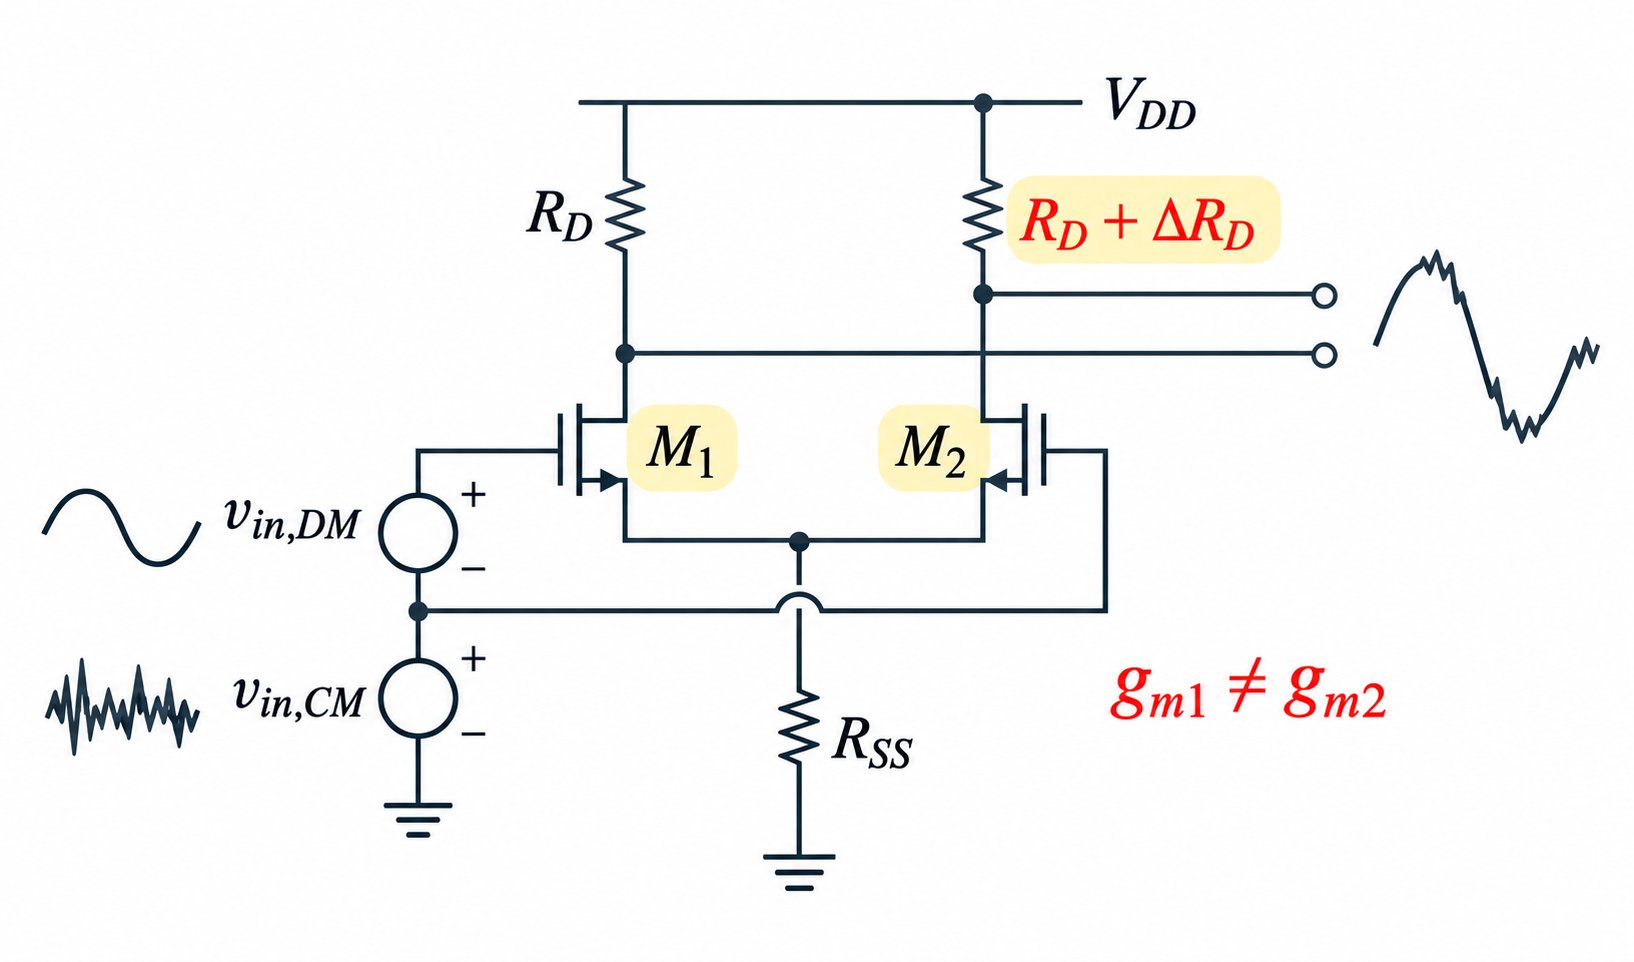
\includegraphics[width=0.5\linewidth,keepaspectratio]{figures/differential-pair-mismatch.png}
    \caption{Differential Pair Mismatch}
    \label{fig:}
\end{minipage}
\par\addvspace{7pt}

\begin{notederivation}[mode=steps,explanation=beside]{CMRR}
    \derivestep{V_{in,CM} \to  V_{od,CM}}{Differential CM mode output due to mismatch}
    \derivestep{A_{V, CM-DM} = \frac{V_{od,CM}}{V_{in,CM}}}{Differential CM and DM Gain}
    \keyequation{Common-mode Rejection Ratio for Simple Differential Pair}{\operatorname{CMRR} = \frac{A_{V,d}}{A_{v,CM-DM}}}
    
\end{notederivation}
\Needspace{85mm}
\noteheading{2}{MOSFET-only differential pairs}
\begingroup
\tcbset{equal height group=mosfet-load-gains}
\begin{notepanels}[gap=7mm,align=top]
    \begin{notepanel}{}
        \begin{notecircuit}[american,scale=0.55,transform shape,
            font=\Large]{Diode-connected load}
            \path[use as bounding box] (-2.95,-3.3) rectangle (5.15,4.1);
            \node[nmos,arrowmos] (DL1) at (0,0) {};
            \node[nmos,arrowmos,xscale=-1] (DL2) at (3.6,0) {};
            \node[pmos,arrowmos] (DL3) at (0,2.55) {};
            \node[pmos,arrowmos,xscale=-1] (DL4) at (3.6,2.55) {};
            \node[right,inner sep=2pt] at (DL1.center) {$M_1$};
            \node[left,inner sep=2pt] at (DL2.center) {$M_2$};
            \node[right,inner sep=2pt] at (DL3.center) {$M_3$};
            \node[left,inner sep=2pt] at (DL4.center) {$M_4$};

            \draw (DL3.S) -- (0,3.7) -- (3.6,3.7) -- (DL4.S);
            \node[right,inner sep=4pt] at (3.6,3.7) {$V_{DD}$};
            \draw (DL3.D) -- (0,1.55) coordinate (dl-diode1)
                -- (0,1.0) coordinate (dl-out1) -- (DL1.D);
            \draw (DL4.D) -- (3.6,1.55) coordinate (dl-diode2)
                -- (3.6,1.0) coordinate (dl-out2) -- (DL2.D);
            \draw (DL3.G) -- (-1.25,2.55) -- (-1.25,1.55)
                -- (dl-diode1) node[circ] {};
            \draw (DL4.G) -- (4.85,2.55) -- (4.85,1.55)
                -- (dl-diode2) node[circ] {};
            \draw[red,densely dashed,line width=0.3pt]
                (-1.5,1.35) rectangle (5.1,3.45);

            \draw (dl-out1) node[circ] {} -- (0.65,1.0) node[ocirc] {};
            \draw (dl-out2) node[circ] {} -- (2.95,1.0) node[ocirc] {};
            \node[left,inner sep=4pt] at (dl-out1) {$X$};
            \node[right,inner sep=4pt] at (dl-out2) {$Y$};
            \node at (1.8,1.0) {$V_{\mathrm{out}}$};
            \node[red] at (0.65,0.63) {$-$};
            \node[red] at (2.95,0.63) {$+$};

            \draw (DL1.S) -- (DL1.S |- 0,-1.0)
                -- (1.8,-1.0) coordinate (dl-source) node[circ] {}
                -- (DL2.S |- 0,-1.0) -- (DL2.S);
            \draw (dl-source) -- (1.8,-1.95)
                to[I,l_=$I_{SS}$] (1.8,-3.05)
                -- ++(0,-0.15) node[ground] {};
            \draw (DL1.G) -- (-1.55,0) node[ocirc] {};
            \node[left] at (-1.55,-0.8) {$V_{\mathrm{in}}$};
            \draw (DL2.G) -- (4.9,0) -- (4.9,-1.65) -- (1.96,-1.65);
            \draw[preaction={draw=white,line width=2pt}]
                (1.64,-1.65) arc[start angle=180,end angle=0,radius=0.16];
            \draw (1.64,-1.65) -- (-1.55,-1.65) node[ocirc] {};
        \end{notecircuit}
        \keyequation{Differential-pair gain\\Diode-connected load}{
            A_v=\frac{g_{m1}}{g_{m3}}
        }
    \end{notepanel}
    \begin{notepanel}{}
        \begin{notecircuit}[american,scale=0.55,transform shape,
            font=\Large]{Current-source load}
            \path[use as bounding box] (-2.95,-3.3) rectangle (5.15,4.1);
            \node[nmos,arrowmos] (CL1) at (0,0) {};
            \node[nmos,arrowmos,xscale=-1] (CL2) at (3.6,0) {};
            \node[pmos,arrowmos,xscale=-1] (CL3) at (0,2.55) {};
            \node[pmos,arrowmos] (CL4) at (3.6,2.55) {};
            \node[right,inner sep=2pt] at (CL1.center) {$M_1$};
            \node[left,inner sep=2pt] at (CL2.center) {$M_2$};
            \node[left,inner sep=3pt] at (CL3.center) {$M_3$};
            \node[right,inner sep=3pt] at (CL4.center) {$M_4$};

            \draw (CL3.S) -- (0,3.7) -- (3.6,3.7) -- (CL4.S);
            \node[right,inner sep=4pt] at (3.6,3.7) {$V_{DD}$};
            \draw (CL3.G) -- (1.8,2.55) coordinate (cl-bias)
                node[circ] {} -- (CL4.G);
            \draw (cl-bias) -- (1.8,3.1) node[ocirc] {}
                node[right,inner sep=3pt] {$V_b$};
            \draw (CL3.D) -- (0,1.0) coordinate (cl-out1) -- (CL1.D);
            \draw (CL4.D) -- (3.6,1.0) coordinate (cl-out2) -- (CL2.D);
            \draw[red,densely dashed,line width=0.3pt]
                (-1.5,1.35) rectangle (5.1,3.45);

            \draw (cl-out1) node[circ] {} -- (0.65,1.0) node[ocirc] {};
            \draw (cl-out2) node[circ] {} -- (2.95,1.0) node[ocirc] {};
            \node[left,inner sep=4pt] at (cl-out1) {$X$};
            \node[right,inner sep=4pt] at (cl-out2) {$Y$};
            \node at (1.8,1.0) {$V_{\mathrm{out}}$};
            \node[red] at (0.65,0.63) {$-$};
            \node[red] at (2.95,0.63) {$+$};

            \draw (CL1.S) -- (CL1.S |- 0,-1.0)
                -- (1.8,-1.0) coordinate (cl-source) node[circ] {}
                -- (CL2.S |- 0,-1.0) -- (CL2.S);
            \draw (cl-source) -- (1.8,-1.95)
                to[I,l_=$I_{SS}$] (1.8,-3.05)
                -- ++(0,-0.15) node[ground] {};
            \draw (CL1.G) -- (-1.55,0) node[ocirc] {};
            \node[left] at (-1.55,-0.8) {$V_{\mathrm{in}}$};
            \draw (CL2.G) -- (4.9,0) -- (4.9,-1.65) -- (1.96,-1.65);
            \draw[preaction={draw=white,line width=2pt}]
                (1.64,-1.65) arc[start angle=180,end angle=0,radius=0.16];
            \draw (1.64,-1.65) -- (-1.55,-1.65) node[ocirc] {};
        \end{notecircuit}
        \keyequation{Differential-pair gain\\Current-source load}{
            A_v=g_{m1}\bigl(r_{o1}\parallel r_{o3}\bigr)
        }
    \end{notepanel}
\end{notepanels}
\endgroup

\noteheading{1}{OTA}
\noteheading{2}{Differential Pair with Active DC Analysis}
\begin{notederivation}[mode=steps,explanation=beside]{DC analysis}
\par\medskip\noindent\begin{minipage}{\linewidth}
\begin{notecircuit}[american,scale=0.55,transform shape,
    font=\Large]{PMOS current-mirror load}
    \ctikzset{current arrow scale=24}
    \tikzset{active-current/.style={red,line width=0.3pt,
        -{Latex[length=2pt,width=1.4pt]}},
        active-load/.style={color=red,densely dashed,
            every node/.append style={solid}}}
    \node[nmos,arrowmos] (AL1) at (0,0) {};
    \node[nmos,arrowmos,xscale=-1] (AL2) at (3.6,0) {};
    \node[pmos,arrowmos,xscale=-1] (AL3) at (0,2.9) {};
    \node[pmos,arrowmos] (AL4) at (3.6,2.9) {};
    \node[nmos,arrowmos] (AL5) at (1.8,-2.0) {};
    \node[right,inner sep=2pt] at (AL1.center) {$M_1$};
    \node[left,inner sep=2pt] at (AL2.center) {$M_2$};
    \node[left,inner sep=3pt] at (AL3.center) {$M_3$};
    \node[right,inner sep=3pt] at (AL4.center) {$M_4$};
    \node[right,inner sep=3pt] at (AL5.center) {$M_5$};

    \draw (AL3.S) -- (0,3.95) -- (3.6,3.95) -- (AL4.S);
    \node[right,inner sep=4pt] at (3.6,3.95) {$V_{DD}$};
    \draw (AL3.D) -- (0,1.45) coordinate (al-feedback) -- (AL1.D);
    \draw (AL4.D) -- (3.6,1.45) coordinate (al-out) -- (AL2.D);
    \coordinate (al-mirror) at (1.8,2.9);
    \draw[note-highlight] (al-feedback) -- (1.8,1.45) -- (al-mirror);
    \draw (AL3.G) -- (al-mirror) node[circ] {} -- (AL4.G);
    \draw (al-feedback) node[circ] {} -- (1.8,1.45) -- (al-mirror);
    \node[left,inner sep=4pt] at (al-feedback) {$F$};

    \draw (AL1.S) -- (AL1.S |- 0,-0.95)
        -- (1.8,-0.95) coordinate (al-source) node[circ] {}
        -- (AL2.S |- 0,-0.95) -- (AL2.S);
    \node[above,inner sep=4pt] at (al-source) {$P$};
    \draw (al-source) -- (AL5.D);
    \draw (AL5.S) -- ++(0,-0.15) node[ground] {};
    \draw (AL5.G) -- ++(-0.35,0) node[ocirc] {} node[left] {$V_b$};
    \draw (AL1.G) -- ++(-0.35,0)
        node[ocirc] {} node[left] {$V_{\mathrm{in1}}$};
    \draw (AL2.G) -- ++(0.35,0)
        node[ocirc] {} node[below,inner sep=4pt] {$V_{\mathrm{in2}}$};

    \draw (al-out) node[circ] {} -- (4.75,1.45) coordinate (al-port)
        node[ocirc] {} node[below,inner sep=4pt] {$V_{\mathrm{out}}$};
    \draw[active-load] (al-port) -- (6.35,1.45)
        to[R,l=$R_L$] (6.35,-0.9)
        -- ++(0,-0.15) node[ground] {};
    \draw[active-current] (-0.55,1.1) -- (-0.55,0.65);
    \node[red,anchor=east,inner sep=0pt] at (-0.8,0.875) {$I_1$};
    \draw[active-current] (4.2,2.4) -- (4.2,1.95);
    \node[red,anchor=west,inner sep=0pt] at (4.45,2.175) {$I_4$};
    \draw[active-current] (3.0,1.05) -- (3.0,0.6);
    \node[red,anchor=east,inner sep=0pt] at (2.75,0.825) {$I_2$};
    \draw[active-current] (5.55,1.85) -- (6.15,1.85);
    \node[red,above,inner sep=4pt] at (5.85,1.85) {$I_{\mathrm{out}}$};
    \draw[active-current] (2.55,-1.05) -- (2.55,-1.55);
    \node[red,anchor=west,inner sep=0pt] at (2.8,-1.3) {$I_5$};
\end{notecircuit}
    \derivestep{I_4 &= I_3 = I_1}{The matched $1{:}1$ mirror formed by $M_3$ and $M_4$ copies the left-branch current.}
\end{minipage}\par

    \par\addvspace{6pt}\Needspace{9\baselineskip}
    \textbf{\boldmath When $V_{\mathrm{in1}}=V_{\mathrm{in2}}$}\par
    \derivestep{
        V_{\mathrm{in1}} &= V_{\mathrm{in2}},\qquad \Delta V_{\mathrm{in}}=0\\
        I_1 &= I_2 = I_3 = I_4 = \frac{I_5}{2}\\
        I_{\mathrm{out}} &= I_4-I_2=0
    }{The tail current splits equally, so the currents entering and leaving the output node cancel.}

    \par\addvspace{6pt}\Needspace{7\baselineskip}
    \textbf{\boldmath $\Delta V_{\mathrm{in}}>0$}\par
    \derivestep{
        \Delta V_{\mathrm{in}} &= V_{\mathrm{in1}}-V_{\mathrm{in2}}>0
    }{The left-branch current increases by $\Delta I$ and the right-branch current decreases by the same amount.}
    \derivestep{
        I_1 &= \frac{I_5}{2}+\Delta I=I_4\\
        I_2 &= \frac{I_5}{2}-\Delta I
    }{The mirror transfers the increase in $I_1$ to $I_4$, while $I_5=I_1+I_2$ remains fixed.}
\end{notederivation}
\keyequation{Output current for a positive differential input}{
    I_{\mathrm{out}}=I_4-I_2
    =\left(\frac{I_5}{2}+\Delta I\right)
    -\left(\frac{I_5}{2}-\Delta I\right)
    =2\Delta I
}

\noteheading{3}{DC output limits}
\begin{notederivation}[mode=steps,explanation=beside]{DC operating cases}
\par\noindent\begin{minipage}{\linewidth}
\begin{notecircuit}[american,scale=0.55,transform shape,
    font=\Large]{Unloaded active-load differential pair}
    \tikzset{dc-current/.style={red,line width=0.3pt,
        -{Latex[length=2pt,width=1.4pt]}},
        dc-guide/.style={blue!70!black,line width=0.3pt,
            -{Latex[length=2pt,width=1.4pt]}}}
    \node[nmos,arrowmos] (DC1) at (0,0) {};
    \node[nmos,arrowmos,xscale=-1] (DC2) at (3.6,0) {};
    \node[pmos,arrowmos,xscale=-1] (DC3) at (0,2.9) {};
    \node[pmos,arrowmos] (DC4) at (3.6,2.9) {};
    \node[nmos,arrowmos] (DC5) at (1.8,-2.0) {};
    \node[right,inner sep=2pt] at (DC1.center) {$M_1$};
    \node[left,inner sep=2pt] at (DC2.center) {$M_2$};
    \node[left,inner sep=3pt] at (DC3.center) {$M_3$};
    \node[right,inner sep=3pt] at (DC4.center) {$M_4$};
    \node[right,inner sep=3pt] at (DC5.center) {$M_5$};

    \draw (DC3.S) -- (0,3.95) -- (3.6,3.95) -- (DC4.S);
    \node[right,inner sep=4pt] at (3.6,3.95) {$V_{DD}$};
    \draw (DC3.D) -- (0,1.45) coordinate (dc-f) -- (DC1.D);
    \draw (DC4.D) -- (3.6,1.45) coordinate (dc-out) -- (DC2.D);
    \coordinate (dc-mirror) at (1.8,2.9);
    \draw[note-highlight] (dc-f) -- (1.8,1.45) -- (dc-mirror);
    \draw (DC3.G) -- (dc-mirror) node[circ] {} -- (DC4.G);
    \draw (dc-f) node[circ] {} -- (1.8,1.45) -- (dc-mirror);
    \node[left,inner sep=4pt] at (dc-f) {$F$};
    \draw (DC1.S) -- (DC1.S |- 0,-0.95)
        -- (1.8,-0.95) coordinate (dc-p) node[circ] {}
        -- (DC2.S |- 0,-0.95) -- (DC2.S);
    \node[above,inner sep=4pt] at (dc-p) {$P$};
    \draw (dc-p) -- (DC5.D);
    \draw (DC5.S) -- ++(0,-0.15) node[ground] {};
    \draw (DC5.G) -- ++(-0.35,0) node[ocirc] {} node[left] {$V_b$};
    \draw (DC1.G) -- ++(-0.35,0)
        node[ocirc] {} node[left] {$V_{\mathrm{in1}}$};
    \draw (DC2.G) -- ++(0.35,0)
        node[ocirc] {} node[below,inner sep=4pt] {$V_{\mathrm{in2}}$};
    \draw (dc-out) node[circ] {} -- (4.75,1.45) node[ocirc] {}
        node[right,inner sep=4pt] {$V_{\mathrm{out}}$};

    \node[blue!70!black,anchor=east,align=right,inner sep=2pt]
        (dc-short) at (-1.55,1.9)
        {{\sffamily Virtual short}\\[2pt]$\Delta V_{\mathrm{in}}=0$};
    \draw[dc-guide] (dc-short.east) to[out=0,in=160] (-0.25,1.55);
    \draw[dc-current] (4.2,2.4) -- (4.2,1.95);
    \node[red,anchor=west,inner sep=0pt] at (4.45,2.175) {$I_4$};
    \draw[dc-current] (4.2,1.05) -- (4.2,0.6);
    \node[red,anchor=west,inner sep=0pt] at (4.45,0.825) {$I_2$};
    \draw[dc-current] (5.55,1.85) -- (6.15,1.85);
    \node[red,above,inner sep=4pt] at (5.85,1.85) {$I_{\mathrm{out}}$};
    \draw[dc-current,orange!85!black] (-0.55,1.05) -- (-0.55,0.6);
    \draw[dc-current,orange!85!black] (2.55,-1.05) -- (2.55,-1.55);
    \node[orange!85!black,anchor=west,inner sep=0pt] at (2.8,-1.3) {$I_5$};
\end{notecircuit}
\par\smallskip{\centering
    $\Delta V_{\mathrm{in}}=0\ \Longrightarrow\ V_F=V_{\mathrm{out}}$\par}
\end{minipage}\par

    \par\addvspace{6pt}\Needspace{8\baselineskip}
    \textbf{\boldmath $\Delta V_{\mathrm{in}}\ll0$}\par
    \derivestep{
        M_1,M_3,M_4&:\ \text{off}\\
        I_4&=0\ \Longrightarrow\ I_2=0\\
        V_{\mathrm{out}}&\to0
    }{The unloaded output falls toward ground; at DC the output-node currents must balance.}

    \par\addvspace{6pt}\Needspace{8\baselineskip}
    \textbf{\boldmath $\Delta V_{\mathrm{in}}=0$}\par
    \derivestep{
        I_1&=I_2=I_3=I_4=\frac{I_5}{2}\\
        I_{\mathrm{out}}&=0\\
        V_{\mathrm{out}}&=V_F=V_{DD}-\lvert V_{GS3}\rvert
    }{The matched branches give $V_F=V_{\mathrm{out}}$; diode-connected $M_3$ sets $V_F$.}

    \par\addvspace{6pt}\Needspace{8\baselineskip}
    \textbf{\boldmath $\Delta V_{\mathrm{in}}\gg0$}\par
    \derivestep{
        M_2&:\ \text{off},\qquad I_2=0\\
        I_{\mathrm{out}}&=I_4,\qquad I_4=I_1=I_3\\
        V_{\mathrm{out}}&\to V_{DD}
    }{The mirror supplies current while $M_4$ remains saturated, raising the unloaded output toward $V_{DD}$; the mirror equality no longer applies at the rail.}
\end{notederivation}
\keyequation{DC output levels}{
    V_{\mathrm{out}}\simeq
    \begin{cases}
        0, & \Delta V_{\mathrm{in}}\ll0,\\[3pt]
        V_{DD}-\lvert V_{GS3}\rvert, & \Delta V_{\mathrm{in}}=0,\\[3pt]
        V_{DD}, & \Delta V_{\mathrm{in}}\gg0.
    \end{cases}
}

\Needspace{70mm}
\noteheading{3}{Large Signal Input-Output Characteristic}
\begin{center}
    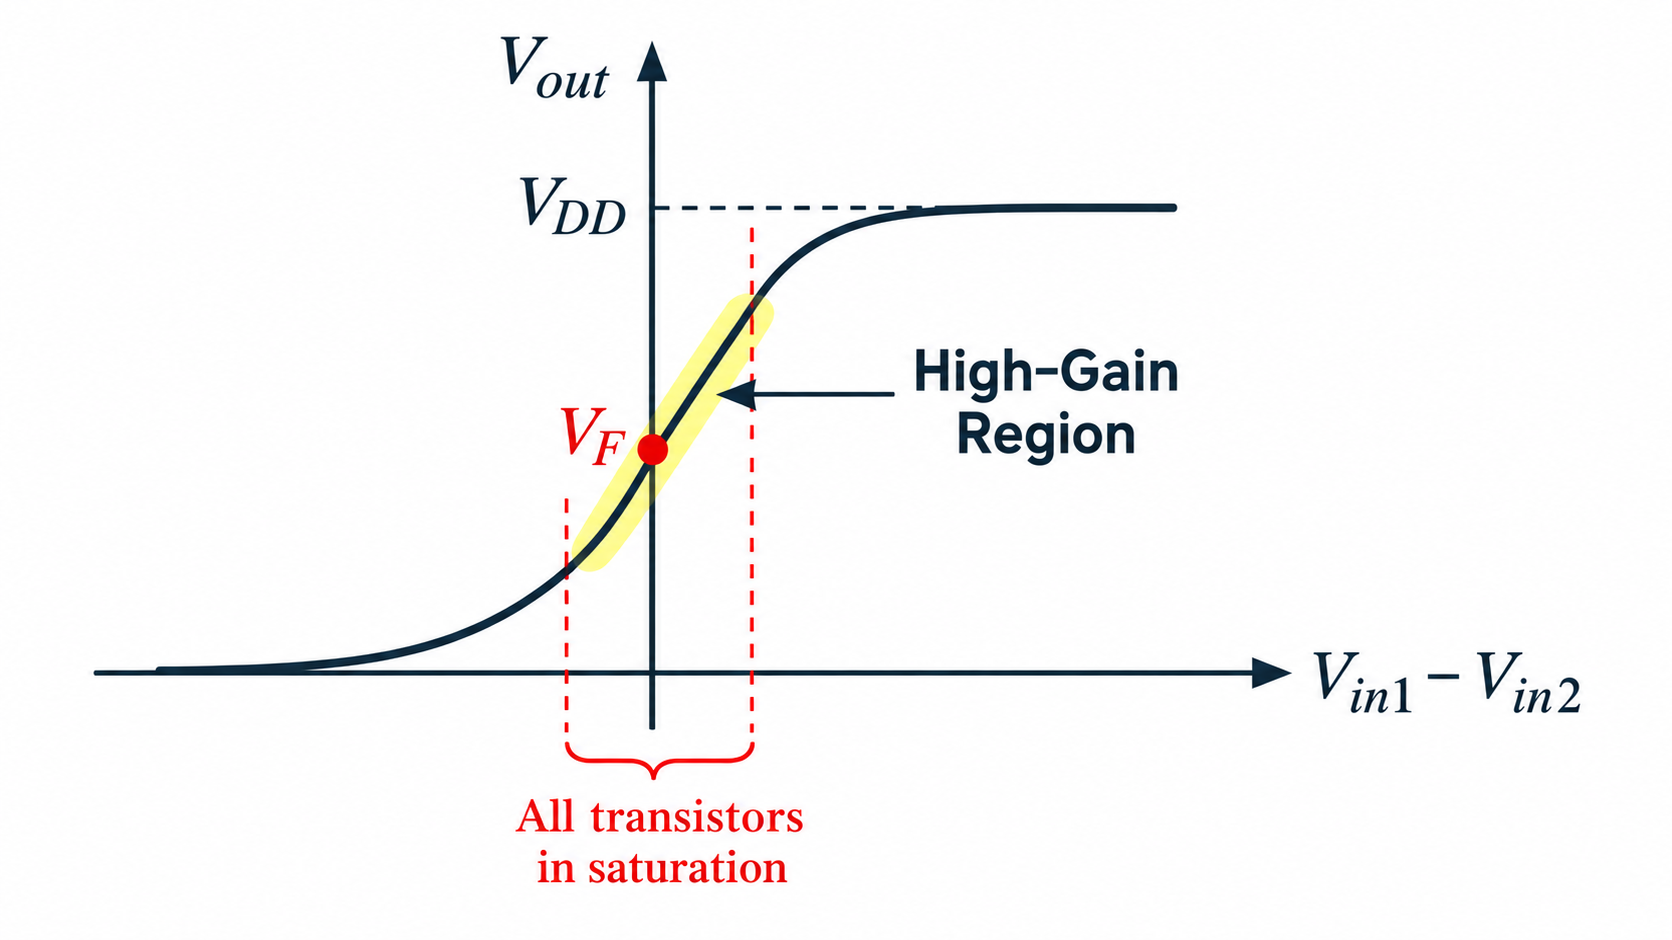
\includegraphics[width=0.55\linewidth,height=65mm,keepaspectratio]{figures/large-signal-input-output-characteristic.png}
\end{center}

\Needspace{85mm}
\noteheading{2}{Common-Mode Input Range}
\begin{notederivation}[mode=steps,explanation=beside]{Common-mode input limits}
\par\noindent\begin{minipage}{\linewidth}
\begin{notecircuit}[american,scale=0.55,transform shape,
    font=\Large]{Common-mode excitation of the active-load pair}
    \tikzset{cm-input/.style={color=red,densely dashed,
        every node/.append style={solid}}}
    \node[nmos,arrowmos] (IR1) at (0,0) {};
    \node[nmos,arrowmos,xscale=-1] (IR2) at (3.6,0) {};
    \node[pmos,arrowmos,xscale=-1] (IR3) at (0,2.9) {};
    \node[pmos,arrowmos] (IR4) at (3.6,2.9) {};
    \node[nmos,arrowmos] (IR5) at (1.8,-2.0) {};
    \node[right,inner sep=2pt] at (IR1.center) {$M_1$};
    \node[left,inner sep=2pt] at (IR2.center) {$M_2$};
    \node[left,inner sep=3pt] at (IR3.center) {$M_3$};
    \node[right,inner sep=3pt] at (IR4.center) {$M_4$};
    \node[right,inner sep=3pt] at (IR5.center) {$M_5$};

    \draw (IR3.S) -- (0,3.95) -- (3.6,3.95) -- (IR4.S);
    \node[right,inner sep=4pt] at (3.6,3.95) {$V_{DD}$};
    \draw (IR3.D) -- (0,1.45) coordinate (ir-f) -- (IR1.D);
    \draw (IR4.D) -- (3.6,1.45) coordinate (ir-out) -- (IR2.D);
    \coordinate (ir-mirror) at (1.8,2.9);
    \draw (IR3.G) -- (ir-mirror) node[circ] {} -- (IR4.G);
    \draw (ir-f) node[circ] {} -- (1.8,1.45) -- (ir-mirror);
    \node[left,inner sep=4pt] at (ir-f) {$F$};
    \draw (ir-out) node[circ] {} -- (4.75,1.45) node[ocirc] {}
        node[right,inner sep=4pt] {$V_{\mathrm{out}}$};

    \draw (IR1.S) -- (IR1.S |- 0,-0.95)
        -- (1.8,-0.95) coordinate (ir-p) node[circ] {}
        -- (IR2.S |- 0,-0.95) -- (IR2.S);
    \node[below right,fill=yellow!40,rounded corners=2pt,inner sep=1.5pt]
        at (ir-p) {$P$};
    \draw (ir-p) -- (IR5.D);
    \draw (IR5.S) -- ++(0,-0.15) node[ground] {};
    \draw (IR5.G) -- ++(-0.35,0) node[ocirc] {} node[left] {$V_b$};

    \draw (IR1.G) -- (-1.5,0) coordinate (ir-gate1) node[circ] {};
    \draw (IR2.G) -- (4.95,0) coordinate (ir-gate2) node[circ] {};
    \node[above,inner sep=4pt] at (ir-gate1) {$V_{\mathrm{in1}}$};
    \node[above,inner sep=4pt] at (ir-gate2) {$V_{\mathrm{in2}}$};
    \draw[cm-input] (ir-gate1) -- (-2.25,0)
        to[V,l_=$V_{\mathrm{in,CM}}$] (-2.25,-1.7)
        -- ++(0,-0.15) node[ground] {};
    \draw[cm-input] (ir-gate1) -- (-1.5,-3.6)
        -- (4.95,-3.6) -- (ir-gate2);
    \node[red] at (1.8,0.7) {$+$};
    \node[red] at (1.8,0.2) {$V_{GS1}$};
    \node[red] at (1.8,-0.3) {$-$};
\end{notecircuit}
    \derivestep{V_{\mathrm{in,CM}}&=V_{GS1}+V_P}{KVL from the common-mode input to the source node $P$.}
\end{minipage}\par

    \par\addvspace{6pt}\Needspace{7\baselineskip}
    \textbf{\boldmath $V_{\mathrm{in,CM,min}}$}\par
    \derivestep{
        V_P&=V_{DS5}\ge V_{OV5}\\
        V_{\mathrm{in,CM}}&\ge V_{GS1}+V_{OV5}\\
        V_{GS1}&=V_{OV1}+V_{TH1}
    }{Keep $M_5$ in saturation; the lower boundary occurs at $V_{DS5}=V_{OV5}$.}

    \par\addvspace{6pt}\Needspace{7\baselineskip}
    \textbf{\boldmath $V_{\mathrm{in,CM,max}}$}\par
    \derivestep{
        V_F-V_P&\ge V_{OV1}\\
        V_F&=V_{DD}-\lvert V_{GS3}\rvert\\
        V_P&=V_{\mathrm{in,CM}}-V_{GS1}
    }{Keep $M_1$ in saturation and use the voltage set by diode-connected $M_3$.}
    \derivestep{
        &V_{DD}-\lvert V_{GS3}\rvert-V_{\mathrm{in,CM}}+V_{GS1}\ge V_{OV1}\\
        &V_{\mathrm{in,CM}}\le V_{DD}+V_{GS1}-\lvert V_{GS3}\rvert-V_{OV1}
    }{Substitute for $V_F$ and $V_P$, then isolate $V_{\mathrm{in,CM}}$.}
\end{notederivation}
\keyequation{Common-mode input voltage limits}{
    \begin{aligned}
        V_{\mathrm{in,CM,min}}&=V_{GS1}+V_{OV5}
            =V_{OV1}+V_{OV5}+V_{TH1}\\[4pt]
        V_{\mathrm{in,CM,max}}&=V_{DD}+V_{GS1}-\lvert V_{GS3}\rvert-V_{OV1}
    \end{aligned}
}

\Needspace{85mm}
\noteheading{2}{Output Swing}
\begin{notederivation}[mode=steps,explanation=beside]{Output voltage limits}
\par\noindent\begin{minipage}{\linewidth}
\begin{notecircuit}[american,scale=0.55,transform shape,
    font=\Large]{Active-load pair with common-mode input}
    \tikzset{swing-input/.style={color=red,densely dashed,
        every node/.append style={solid}}}
    \node[nmos,arrowmos] (SW1) at (0,0) {};
    \node[nmos,arrowmos,xscale=-1] (SW2) at (3.6,0) {};
    \node[pmos,arrowmos,xscale=-1] (SW3) at (0,2.9) {};
    \node[pmos,arrowmos] (SW4) at (3.6,2.9) {};
    \node[nmos,arrowmos] (SW5) at (1.8,-2.0) {};
    \node[right,inner sep=2pt] at (SW1.center) {$M_1$};
    \node[left,inner sep=2pt] at (SW2.center) {$M_2$};
    \node[left,inner sep=3pt] at (SW3.center) {$M_3$};
    \node[right,inner sep=3pt] at (SW4.center) {$M_4$};
    \node[right,inner sep=3pt] at (SW5.center) {$M_5$};

    \draw (SW3.S) -- (0,3.95) -- (3.6,3.95) -- (SW4.S);
    \node[right,inner sep=4pt] at (3.6,3.95) {$V_{DD}$};
    \draw (SW3.D) -- (0,1.45) coordinate (sw-f) -- (SW1.D);
    \draw (SW4.D) -- (3.6,1.45) coordinate (sw-out) -- (SW2.D);
    \coordinate (sw-mirror) at (1.8,2.9);
    \draw (SW3.G) -- (sw-mirror) node[circ] {} -- (SW4.G);
    \draw (sw-f) node[circ] {} -- (1.8,1.45) -- (sw-mirror);
    \node[left,inner sep=4pt] at (sw-f) {$F$};
    \draw (sw-out) node[circ] {} -- (4.75,1.45) node[ocirc] {}
        node[right,inner sep=4pt] {$V_{\mathrm{out}}$};

    \draw (SW1.S) -- (SW1.S |- 0,-0.95)
        -- (1.8,-0.95) coordinate (sw-p) node[circ] {}
        -- (SW2.S |- 0,-0.95) -- (SW2.S);
    \node[above,inner sep=4pt] at (sw-p) {$P$};
    \draw (sw-p) -- (SW5.D);
    \draw (SW5.S) -- ++(0,-0.15) node[ground] {};
    \draw (SW5.G) -- ++(-0.35,0) node[ocirc] {} node[left] {$V_b$};
    \draw (SW1.G) -- ++(-0.35,0) node[ocirc] {}
        node[left] {$V_{\mathrm{in1}}$};
    \draw (SW2.G) -- (4.95,0) coordinate (sw-in) node[circ] {}
        node[above,inner sep=4pt] {$V_{\mathrm{in2}}$};
    \draw[swing-input] (sw-in) -- (5.6,0)
        to[V,l=$V_{\mathrm{in,CM}}$] (5.6,-1.7)
        -- ++(0,-0.15) node[ground] {};
    \node[blue!70!black] at (4.95,-0.4) {$+$};
    \node[blue!70!black] at (1.2,-1.2) {$-$};
    \node[blue!70!black] at (2.55,-1.3) {$+$};
    \node[blue!70!black] at (2.55,-2.85) {$-$};
\end{notecircuit}

    \par\addvspace{6pt}\textbf{\boldmath $V_{\mathrm{out,max}}$}\par
    \derivestep{
        V_{DD}-V_{\mathrm{out}}&\ge V_{OV4}\\
        V_{\mathrm{out}}&\le V_{DD}-V_{OV4}
    }{Keep PMOS $M_4$ in saturation: $V_{SD4}\ge V_{OV4}$.}
\end{minipage}\par

    \par\addvspace{6pt}\Needspace{7\baselineskip}
    \textbf{\boldmath $V_{\mathrm{out,min}}$}\par
    \derivestep{
        V_{\mathrm{out}}-V_P&\ge V_{\mathrm{in,CM}}-V_P-V_{TH2}\\
        V_{\mathrm{out}}&\ge V_{\mathrm{in,CM}}-V_{TH2}
    }{Keep $M_2$ in saturation: $V_{DS2}\ge V_{OV2}$, with $V_{GS2}=V_{\mathrm{in,CM}}-V_P$.}
    \derivestep{
        V_{\mathrm{in,CM,min}}&=V_{GS2}+V_{OV5}
    }{At the minimum common-mode input, $M_5$ is at the saturation boundary, so $V_P=V_{OV5}$.}
    \derivestep{
        V_{\mathrm{out,min}}&=V_{GS2}+V_{OV5}-V_{TH2}\\
        &=V_{OV2}+V_{TH2}+V_{OV5}-V_{TH2}\\
        &=V_{OV2}+V_{OV5}
    }{Set $V_{\mathrm{in,CM}}=V_{\mathrm{in,CM,min}}$ and substitute $V_{GS2}=V_{OV2}+V_{TH2}$.}
\end{notederivation}
\keyequation{Output swing limits}{
    \begin{aligned}
        V_{\mathrm{out,max}}&=V_{DD}-V_{OV4}\\[4pt]
        V_{\mathrm{out,min}}&=V_{OV2}+V_{OV5}
            \quad\bigl(V_{\mathrm{in,CM}}=V_{\mathrm{in,CM,min}}\bigr)
    \end{aligned}
}

\end{document}
